\documentclass[conference]{IEEEtran}

\usepackage{amsmath,amssymb}
\usepackage{stmaryrd}
\usepackage{amsthm}
\usepackage{booktabs}
\usepackage{tikz}
\usepackage{quantikz}
\usepackage{algorithm}
\usepackage{algpseudocode}
\usepackage[hidelinks]{hyperref}

\newcommand{\code}[1]{\texttt{#1}}
\newcommand{\Algo}[1]{\textup{\textsc{#1}}}

\theoremstyle{plain}
\newtheorem{theorem}{Theorem}
\newtheorem{lemma}{Lemma}

\begin{document}

\title{From Truth Table to Quantum Circuit:\\K-Map-Guided Toffoli Synthesis}
\author{\IEEEauthorblockN{Arham Akhtar}
\IEEEauthorblockA{Lightrider\\
Bangalore, India\\
aakhtar@lightriderinc.com}}

\maketitle

\begin{abstract}
Karnaugh-map grouping is unsound when applied unchanged to reversible
circuits: a classical AND-OR circuit \emph{sets} its output, but a
Toffoli circuit \emph{flips} it, so a cell covered by two groups is
flipped back to $0$. We prove that a Toffoli circuit built from cubes is
correct exactly when every cell is covered an odd number of times if the
function is $1$ there and an even number of times otherwise. Disjoint
covers, grown greedily on the K-map, are the simplest such covers;
fixed-polarity Reed--Muller forms and a term-merging rule give
overlapping ones. Three function-preserving passes, each with a proof,
shrink every candidate: deriving one output from another, cancelling
adjacent $X$ gates, and reordering terms so that more $X$ gates cancel.
Every candidate is checked by exhaustive simulation, transpiled to a
model of a 133-qubit IBM device and checked again, and the one with the
fewest CZ gates is kept. On eleven functions of two to eight inputs,
disjoint covers alone are not competitive: tweedledum's ESOP circuits
have fewer gates on eight functions and need fewer CZ gates on seven.
With overlapping covers, our circuits need fewer CZ gates than
tweedledum's better circuit on six functions, as many on four, and more
on one (\texttt{3\_17}, $49$ vs.\ $44$). Published in-place circuits for
\texttt{3\_17} and \texttt{rd32} remain $2.0\times$ and $1.5\times$
smaller.
\end{abstract}

\begin{IEEEkeywords}
reversible logic synthesis, Karnaugh maps, Toffoli gates, disjoint cube
cover, ESOP, Reed--Muller, quantum circuit synthesis, quantum cost
\end{IEEEkeywords}

\section{Introduction}
Grover oracles must flip a target qubit iff a classical predicate
$f(x)=1$, and Shor-style arithmetic chains one-bit adders; both need
correct reversible circuits built from truth tables. The textbook tool
for minimizing such logic, the Karnaugh map~\cite{karnaugh1953}, allows
overlapping groups. That is sound for a gate that sets its output but
not for one that XORs into it: for $\mathrm{Out}=A+B$, the naive circuit
\code{cx(B,Out)}; \code{cx(A,Out)} returns $0$ on $A{=}B{=}1$.

Our contributions are: (1) a parity condition under which any cube
cover gives a correct Toffoli circuit, with a greedy algorithm for exact
disjoint covers on the K-map and overlapping covers from fixed-polarity
Reed--Muller forms and term merging; (2) output derivation,
$X$-cancellation, and term reordering, each proved function-preserving,
with derivation chosen by the gate count left after cancellation;
(3) selection among checked candidates by CZ count on an IBM device
model, and an evaluation on eleven functions against published RevLib
circuits and tweedledum, which reports where our circuits are larger. The code that produces every number here is at
\url{https://github.com/ArhamAkhtarAlam/toffoli-synthesis-final-paper}.

\section{Related Work}
Reversible synthesis from truth tables~\cite{saeedi2013} includes
transformation-based synthesis~\cite{miller2003}, ESOP-based synthesis
(e.g.\ EXORCISM-4~\cite{mishchenko2001}), BDD-based
synthesis~\cite{wille2009bdd}, and exact SAT-based
synthesis~\cite{grosse2008}. Our covers are ESOPs: the disjoint ones are a
restricted ESOP with a one-line correctness proof, and fixed-polarity
Reed--Muller forms~\cite{saeedi2013} are a classical source of
overlapping ones (tweedledum's PPRM is the positive-polarity case). RevLib~\cite{revlib2008} collects
benchmarks and published circuits; RevKit~\cite{soeken2012revkit} and
tweedledum~\cite{schmitt2022} implement these synthesis families, and
Qiskit~\cite{qiskit2024} exposes truth-table oracles; its transpiler
maps our circuits to a device's gates and connectivity.

\section{Covers and Circuits}
A \emph{pattern} $p\in\{0,1,-\}^n$ denotes the cube $\llbracket
p\rrbracket=\{x : x_k=p_k \text{ whenever } p_k\neq -\}$. Circuits act
on $n$ input, $m$ output, and $a$ ancilla wires (outputs and ancillas
start at $0$) with gates $X$ and $C^kX$ (flip the target iff all $k$
controls are $1$): the positive-control MCT library of
RevLib~\cite{revlib2008}. A term $p$ becomes one $C^kX$ on the wires
where $p$ is specified, wrapped in $X$ gates on those where $p_k=0$, so
it flips its target iff $x\in\llbracket p\rrbracket$. The quantum cost
of a $C^kX$ is $2^{k+1}-3$ ($1$ for $X$ and CNOT)~\cite{barenco1995,revlib2008}.

A K-map lays out a truth table so that adjacent cells differ in one bit;
a group of $2^d$ adjacent $1$-cells is a cube with $d$ dashes.
Classical grouping lets groups overlap, but a Toffoli circuit flips a cell
once per group containing it, so a cell in two groups ends at $0$ (cell
$11$ of $A+B$). Overlaps are harmless only when every cell is covered an
odd number of times, as for Carry's three pairs, which meet only at
$111$ (Theorem~\ref{thm:correctness}). Algorithm~\ref{alg:cover}
avoids overlaps: it grows each group only inside the cells not yet
covered (Fig.~\ref{fig:kmaps}).

\begin{figure}[t]
\centering
\begin{minipage}{0.48\linewidth}
\centering
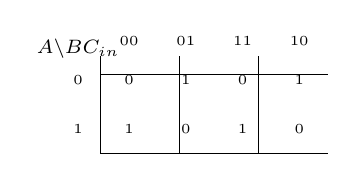
\begin{tikzpicture}[x=0.72cm,y=0.62cm,font=\tiny]
  \draw (0,0) grid (4,2);
  \node at (0.5,2.3) {$00$}; \node at (1.5,2.3) {$01$};
  \node at (2.5,2.3) {$11$}; \node at (3.5,2.3) {$10$};
  \node at (0.5,1.5) {$0$}; \node at (1.5,1.5) {$1$};
  \node at (2.5,1.5) {$0$}; \node at (3.5,1.5) {$1$};
  \node at (0.5,0.5) {$1$}; \node at (1.5,0.5) {$0$};
  \node at (2.5,0.5) {$1$}; \node at (3.5,0.5) {$0$};
  \node at (-0.4,1.5) {$0$}; \node at (-0.4,0.5) {$1$};
  \node at (-0.4,2.15) {\scriptsize $A{\backslash}BC_{in}$};
\end{tikzpicture}
\par\vspace{2pt}{\scriptsize Sum: no two 1-cells adjacent (parity).}
\end{minipage}
\hfill
\begin{minipage}{0.48\linewidth}
\centering
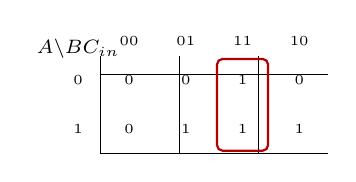
\begin{tikzpicture}[x=0.72cm,y=0.62cm,font=\tiny]
  \draw (0,0) grid (4,2);
  \node at (0.5,2.3) {$00$}; \node at (1.5,2.3) {$01$};
  \node at (2.5,2.3) {$11$}; \node at (3.5,2.3) {$10$};
  \node at (0.5,1.5) {$0$}; \node at (1.5,1.5) {$0$};
  \node at (2.5,1.5) {$1$}; \node at (3.5,1.5) {$0$};
  \node at (0.5,0.5) {$0$}; \node at (1.5,0.5) {$1$};
  \node at (2.5,0.5) {$1$}; \node at (3.5,0.5) {$1$};
  \node at (-0.4,1.5) {$0$}; \node at (-0.4,0.5) {$1$};
  \node at (-0.4,2.15) {\scriptsize $A{\backslash}BC_{in}$};
  \draw[thick,red!70!black,rounded corners=2pt] (2.05,0.06) rectangle (2.95,1.94);
\end{tikzpicture}
\par\vspace{2pt}{\scriptsize Carry: group $BC_{in}$; the other two 1-cells must be single terms.}
\end{minipage}
\caption{K-maps for the full adder. No two of Sum's $1$-cells are adjacent; Carry's disjoint cover is the boxed pair and two single cells.}
\label{fig:kmaps}
\end{figure}

\begin{algorithm}[t]
\caption{\Algo{DisjointCover}$(S)$}
\label{alg:cover}
\begin{algorithmic}[1]
\State $R \gets S$; $T\gets\langle\rangle$
\While{$R \ne \emptyset$}
  \State $p \gets \min(R)$
  \For{$i \gets 1$ \textbf{to} $n$}\Comment{\Algo{GrowCube}}
    \State \textbf{if} $\llbracket p \text{ with } p_i{=}{-}\rrbracket \subseteq R$ \textbf{then} $p_i \gets -$
  \EndFor
  \State append $p$ to $T$; $R \gets R\setminus\llbracket p\rrbracket$
\EndWhile
\State \Return $T$
\end{algorithmic}
\end{algorithm}

\begin{theorem}[Exact, disjoint cover]
\label{thm:exactness}
The cubes returned by Algorithm~\ref{alg:cover} are pairwise disjoint and
their union is $S$.
\end{theorem}
\begin{proof}
Each cube is grown only while it stays inside the current remainder $R$,
which excludes all earlier cubes, so cubes are disjoint and lie in $S$.
Each iteration removes at least its seed, so the loop ends, with $R=\emptyset$,
after at most $|S|$ iterations.
\end{proof}

\begin{theorem}[Correct synthesis]
\label{thm:correctness}
Emitting terms $p_1,\dots,p_t$ onto output wire $j$ leaves $f_j(x)$ on it,
for every input $x$, iff $|\{i : x\in\llbracket p_i\rrbracket\}|$ is odd
exactly when $f_j(x)=1$. In particular, \Algo{DisjointCover}$(f_j)$
does.
\end{theorem}
\begin{proof}
A term flips wire $j$ iff $x$ is in its cube, and flips add mod $2$. No
gate targets an input wire. Disjoint cubes covering the on-set
(Theorem~\ref{thm:exactness}) contain each on-cell once and each
off-cell never.
\end{proof}

Fig.~\ref{fig:fulladder} shows the full adder: $4$ singleton terms for
$\mathrm{Sum}$ (parity admits no larger cube) and $3$ for
$\mathrm{Carry}$, $23$ gates in all.

\textbf{Overlapping covers.} For a polarity $\pi\in\{0,1\}^n$, the
fixed-polarity Reed--Muller (FPRM) form writes $f_j$ as an XOR of
products of the literals $x_i$ ($\pi_i=0$) or $\bar x_i$ ($\pi_i=1$);
its coefficients follow from the truth table by a butterfly transform in
$O(n2^n)$. Each product is a cube, and the form is an identity, so each
of the $2^n$ FPRM forms satisfies Theorem~\ref{thm:correctness}
($\pi=0^n$ is the PPRM). For the full adder, $\mathrm{Sum}=A\oplus
B\oplus C_{in}$ is three CNOTs instead of four 3-control terms.
\begin{lemma}[Merging]
\label{lem:merge}
Two cubes that differ in one position $i$ can be replaced by the cube
with the third value of $\{0,1,-\}$ at $i$; two equal cubes can be
deleted. Neither changes the parity in Theorem~\ref{thm:correctness}.
\end{lemma}
\begin{proof}
With $c$ the common part, $c x_i\oplus c\bar x_i=c$, $c\oplus cx_i=c\bar
x_i$, $c\oplus c\bar x_i=cx_i$, and $c\oplus c=0$.
\end{proof}
Merging removes a term but can add negated literals ($X$ gates), so
both versions of each cover are kept. The candidate covers of an output
are Algorithm~\ref{alg:cover} under every variable order ($2n$
rotations and reversals for $n>4$) with the smallest or largest seed,
all FPRM forms, and each of these merged.

\begin{figure}[t]
\centering
\resizebox{\columnwidth}{!}{%
\begin{quantikz}[column sep=4pt, row sep={0.8cm,between origins}]
\lstick{$A$} & \gate{X} & \ctrl{1} & \gate{X}\gategroup[wires=1,steps=2,style={dashed,rounded corners,thick,draw=red!75!black,inner xsep=2pt,inner ysep=1pt}]{} & \gate{X} & \ctrl{1} & \gate{X} & \qw & \ctrl{1} & \qw & \ctrl{1} & \qw & \qw & \ctrl{1} & \qw & \qw & \ctrl{1} & \qw & \qw \\
\lstick{$B$} & \gate{X} & \ctrl{1} & \gate{X} & \qw & \ctrl{1} & \qw & \gate{X} & \ctrl{1} & \gate{X} & \ctrl{1} & \ctrl{1} & \gate{X} & \ctrl{1} & \gate{X} & \qw & \ctrl{1} & \qw & \qw \\
\lstick{$C_{in}$} & \qw & \ctrl{1} & \qw & \gate{X} & \ctrl{1} & \gate{X}\gategroup[wires=1,steps=2,style={dashed,rounded corners,thick,draw=red!75!black,inner xsep=2pt,inner ysep=1pt}]{} & \gate{X} & \ctrl{1} & \gate{X} & \ctrl{1} & \ctrl{2} & \qw & \ctrl{2} & \qw & \gate{X} & \ctrl{2} & \gate{X} & \qw \\
\lstick{$\mathrm{Sum}=\ket0$} & \qw & \targ{} & \qw & \qw & \targ{} & \qw & \qw & \targ{} & \qw & \targ{} & \qw & \qw & \qw & \qw & \qw & \qw & \qw & \qw \\
\lstick{$\mathrm{Carry}=\ket0$} & \qw & \qw & \qw & \qw & \qw & \qw & \qw & \qw & \qw & \qw & \targ{} & \qw & \targ{} & \qw & \qw & \targ{} & \qw & \qw
\end{quantikz}}
\caption{Full adder as emitted: $\mathrm{Sum}$'s four terms, then
$\mathrm{Carry}$'s three ($23$ gates). In each dashed box, one term ends
and the next begins with an $X$ on the same wire, and no gate between
them uses that wire as a control; since $XX=I$, both are deleted
(Lemma~\ref{lem:xcancel}), leaving $19$ gates.}
\label{fig:fulladder}
\end{figure}

\begin{table*}[t]
\centering
\caption{Gates after $X$-cancellation (Raw: one term per on-set row, before cancellation; disjoint cover; disjoint
pipeline with term ordering; hybrid), and gates, quantum cost, and CZ count on the IBM Heron model for the
disjoint pipeline (Disj.), the hybrid (Hyb.: the checked candidate with the fewest CZ gates), and tweedledum's
PKRM and PPRM circuits, all on the same $n+m$ lines.}
\label{tab:results}
\footnotesize
\setlength{\tabcolsep}{4pt}
\begin{tabular}{@{}lrr rrrr rr rrrr rrrr@{}}
\toprule
& & & \multicolumn{4}{c}{This work: gates} & \multicolumn{2}{c}{tweedledum gates} & \multicolumn{4}{c}{$Q$-cost} & \multicolumn{4}{c}{CZ on device}\\
\cmidrule(lr){4-7}\cmidrule(lr){8-9}\cmidrule(lr){10-13}\cmidrule(l){14-17}
Function & $n$ & $m$ & Raw & Cover & Disj. & Hyb. & PKRM & PPRM & Disj. & Hyb. & PKRM & PPRM & Disj. & Hyb. & PKRM & PPRM\\
\midrule
AND & 2 & 1 & 1 & 1 & 1 & 1 & 1 & 1 & 5 & 5 & 5 & 5 & 7 & 7 & 7 & 7\\
OR & 2 & 1 & 7 & 4 & 4 & 4 & 4 & 3 & 8 & 8 & 8 & 7 & 7 & 7 & 10 & 8\\
XOR & 2 & 1 & 6 & 6 & 6 & 2 & 2 & 2 & 14 & 2 & 2 & 2 & 17 & 2 & 2 & 2\\
NAND & 2 & 1 & 11 & 6 & 6 & 2 & 6 & 2 & 10 & 6 & 10 & 6 & 7 & 7 & 8 & 7\\
Half adder & 2 & 2 & 7 & 7 & 6 & 3 & 3 & 3 & 14 & 7 & 7 & 7 & 19 & 12 & 14 & 14\\
Full adder (\texttt{rd32}) & 3 & 2 & 26 & 19 & 14 & 6 & 10 & 6 & 74 & 18 & 22 & 18 & 133 & 34 & 34 & 36\\
2-bit ripple adder & 5 & 4 & 332 & 86 & 31 & 16 & 34 & 18 & 411 & 104 & 142 & 118 & 514 & 206 & 243 & 231\\
BCD to Excess-3 & 4 & 4 & 122 & 36 & 22 & 24 & 45 & 32 & 190 & 140 & 257 & 292 & 279 & 197 & 388 & 493\\
$3{\times}3$ multiplier & 6 & 6 & 615 & 123 & 60 & 27 & 80 & 27 & 1920 & 627 & 936 & 919 & 2058 & 724 & 1235 & 1039\\
4-bit equality & 8 & 1 & 144 & 76 & 52 & 24 & 24 & 81 & 8180 & 472 & 472 & 1009 & 7534 & 699 & 752 & 1768\\
\texttt{3\_17} & 3 & 3 & 48 & 22 & 13 & 12 & 15 & 14 & 37 & 28 & 31 & 30 & 65 & 49 & 44 & 49\\
\bottomrule
\end{tabular}
\end{table*}

\section{Optimizations}
\textbf{Derivation.} A later output $f_k$ may be built as a CNOT from an
earlier output wire $j$ followed by a cover of $r=f_j\oplus f_k$.
\begin{lemma}[Derivation]
\label{lem:derive}
If wire $j$ holds $f_j(x)$, a CNOT $j\to k$ followed by the terms of a
cover of $r$ that satisfies Theorem~\ref{thm:correctness} leaves
$f_k(x)$ on $k$ and changes no other wire.
\end{lemma}
\begin{proof}
Wire $k$ ends at $f_j(x)\oplus r(x)=f_k(x)$ by
Theorem~\ref{thm:correctness} applied to $r$.
\end{proof}
On a two-bit ripple adder ($S_0,C_0,S_1,\mathrm{Cout}$) derivation finds
$S_1\oplus C_0=A_1\oplus B_1$, the identity ``sum $=$ inputs XOR carry,''
and cuts its disjoint circuit from $126$ gates to $64$. A term common to several outputs can also
be computed once into an ancilla, copied, and uncomputed; for two
outputs this costs $2c+2$ gates against $2c$, so it almost never pays
and no circuit here uses it.


\textbf{$X$-cancellation.} Adjacent terms often leave $X_w\cdots X_w$ on
an input wire $w$, as in the two boxed pairs of Fig.~\ref{fig:fulladder}.
\begin{lemma}[$X$-cancellation]
\label{lem:xcancel}
If no gate between two $X_w$ uses $w$ as a control, deleting both leaves
the circuit's action unchanged.
\end{lemma}
\begin{proof}
$X_w$ commutes with gates not involving $w$ and with gates targeting
$w$ (both flip $w$; their condition does not depend on $w$), so the two
$X_w$ become adjacent and $X_wX_w=I$.
\end{proof}
Since $X$ gates sit only on inputs, the cancelled length is the number
of $C^kX$ gates plus, per wire, the parity of the $X$ gates between
consecutive control uses, computed in one pass. Chosen by gate count
\emph{before} cancellation, derivation can hurt: the full adder goes
from $19$ (cancellation alone) to $22$. We therefore score each
derivation candidate by the cancelled length of the circuit so far, and
fall back to the plain cover whenever it is shorter, so the pipeline is
never worse than cover plus cancellation. On the ripple adder this
derives $\mathrm{Cout}$ instead of $S_0$ from $C_0$: one gate more before
cancellation, but $47$ gates after it instead of $58$.

\textbf{Term ordering.} Call each term's gates, and each derivation CNOT,
a \emph{block}.
\begin{lemma}[Reordering]
\label{lem:reorder}
Any block order in which each derivation CNOT from output $i$ follows
every block writing wire $i$ computes the same function.
\end{lemma}
\begin{proof}
Each block XORs a function of wires it does not write into the wires it
writes, so two blocks commute unless one writes a wire the other reads;
only a derivation CNOT reads a non-input wire. Any order meeting the
constraint is reached from the emitted one by swapping adjacent
commuting blocks.
\end{proof}
Our heuristic builds an order greedily (append the admissible block that
gives the shortest cancelled prefix), then moves single blocks while the
cancelled length drops. For reference, dynamic programming over
(placed blocks, per-wire $X$ parity) gives the exact optimum in
$O(2^B2^nB)$ for $B$ blocks; for the full adder's cover it matches
exhaustive search over all $7!$ orders ($15$ gates).

\textbf{Selection.} Each output, and each derivation difference $r$,
takes its cheapest candidate cover, by gates or by quantum cost after
cancellation, from three pools: disjoint covers; all covers; disjoint and
FPRM covers in merged form only. Each of these six rules, and the
disjoint pipeline itself, yields a circuit after derivation,
cancellation, and ordering; each is checked on all inputs and
transpiled, and the one with the fewest CZ gates is kept. The disjoint
pipeline is a candidate, so the hybrid is never worse on the device.


\section{Evaluation}
\textbf{Setup.} The method is implemented in Python. The functions are
the six built-in presets (AND, OR, XOR, NAND, half and full adder), a
two-bit ripple adder with all four internal signals as outputs,
BCD-to-Excess-3, a $3\times3$-bit multiplier, a 4-bit equality
comparator (the shape of a Grover oracle predicate), and RevLib's
\texttt{3\_17}~\cite{revlib2008}. Every circuit, before and after each
pass, is checked against its truth table on all $2^n$ inputs by classical
replay, which is exact because every gate maps basis states to basis
states. Algorithm~\ref{alg:cover} was also checked on $2000$ random
on-sets ($n\le6$) with no overlap or gap. Over $2000$ random truth tables
($2\le n\le4$, $1\le m\le3$), cancellation shortens $47.2\%$ of cover
circuits ($9.7\%$ on average); without the post-cancellation choice the
pipeline is worse than cover plus cancellation in $2.4\%$ of them, and
with it in none; ordering removes a further $9.4\%$ and reaches the
exact optimum in $94.9\%$ of the $1904$ circuits where that optimum was
computed. Derivation is used in $48.7\%$ of the $1326$ tables with two
or more outputs, cutting gates before cancellation by $22.5\%$ when
used; sharing is chosen in $0.4\%$. The checker accepted every circuit
and rejected each one against its table with one output bit flipped.
Choosing, without a transpiler, the candidate with the fewest gates
among those no worse than the disjoint pipeline in gates and quantum
cost, the hybrid is smaller than the disjoint pipeline on
$76.3\%$ of the $1907$ non-empty tables ($22.6\%$ fewer gates and
$25.1\%$ lower quantum cost on average) and larger on none; other
disjoint covers alone help on $11.1\%$ ($1.1\%$).

\textbf{Disjoint pipeline.} Table~\ref{tab:results} shows the passes
compounding: the multiplier goes from $615$ to $60$ gates. On the comparator no cube
larger than a minterm exists, so the whole gain ($144\to52$) comes from
cancellation and ordering; ordering stops at $52$ there against an exact
$48$.

\textbf{tweedledum.} We ran tweedledum~1.1.1~\cite{schmitt2022}'s PKRM
and PPRM synthesizers, which build each output as an ESOP on its own
line, rewrote negative controls as $X$-sandwiches, applied our
cancellation pass, and verified each circuit. Its better circuit has
fewer gates than our disjoint pipeline on eight functions; ours has
fewer only on BCD-to-Excess-3 ($22$ vs.\ $32$) and \texttt{3\_17} ($13$
vs.\ $14$), and lower quantum cost only on BCD-to-Excess-3. The
comparator is the worst case ($Q$-cost $8180$ vs.\ $472$): each of its
disjoint terms is an 8-control minterm, while an ESOP shares structure
across terms.

\textbf{Hybrid.} Allowing overlaps closes most of the gap. Choosing each
output's cover by gate count, without derivation, the ripple adder, multiplier, and
\texttt{3\_17} come out at exactly PPRM's $18$, $27$, and $14$ gates;
derivation takes them to $16$, $25$, and $12$. Table~\ref{tab:results}
lists the hybrid circuit with the fewest CZ gates: it has fewer gates
than tweedledum's better circuit on three functions, as many on seven,
and one more on OR. Fewer gates do not always mean fewer CZ gates: the
3-gate OR needs $9$ against the 4-gate circuit's $7$, and the 25-gate
multiplier $1012$ against the 27-gate one's $724$, so selection keeps
the latter.

\textbf{Published circuits.} For the bijection \texttt{3\_17}, RevLib
lists a Miller--Maslov--Dueck circuit~\cite{miller2003} with $6$ gates
($Q$-cost $14$) on $3$ lines and an exact elementary-gate circuit with
$Q$-cost $10$~\cite{grosse2008}; tweedledum's transformation-based
synthesis gives $7$ gates ($Q$-cost $15$). For \texttt{rd32}, the full
adder, the best listed MCT circuit has $4$ gates ($Q$-cost $12$) on $4$
lines. Our disjoint circuits are $2.2\times$ and $3.5\times$ larger in
gates and $2.6\times$ and $6.2\times$ in quantum cost, the hybrid ones
$2.0\times$ and $1.5\times$ in both, partly because they are
out-of-place ($n+m$ lines, inputs preserved) while the published ones
are in-place or keep garbage. These circuits are quoted from RevLib,
not re-run.

\textbf{On a device.} We transpiled every circuit with Qiskit~2.6 to
FakeTorino, Qiskit's offline model of the 133-qubit IBM Heron processor
\texttt{ibm\_torino} (native CZ, $\sqrt{X}$, $R_z$; its coupling map),
at optimization level 3 with a fixed seed, and checked each transpiled
circuit, placement and routing included, by statevector simulation on
all inputs. The transpiler must be told that qubits do not start in
$\ket0$: by default it borrows untouched input wires as clean scratch
qubits, and the transpiled ripple adder is then wrong on some inputs.
Our disjoint circuits need fewer CZ gates than tweedledum's better one
only on OR and BCD-to-Excess-3 ($279$ vs.\ $388$), tie on AND and NAND,
and need more on the other seven. Which circuit needs fewer CZ gates
matches which has lower quantum cost in $18$ of the $22$ comparisons,
and which has fewer MCT gates in only $13$: on \texttt{3\_17} ours has
fewer gates but $65$ CZ gates against $44$. Quantum cost is the better
proxy. The hybrid needs fewer CZ gates than tweedledum's better circuit
on six functions (e.g.\ $206$ vs.\ $231$ for the ripple adder, $724$
vs.\ $1039$ for the multiplier, $197$ vs.\ $388$ for BCD-to-Excess-3),
as many on AND, XOR, NAND, and the full adder, and more only on
\texttt{3\_17} ($49$ vs.\ $44$).

\section{Limitations and Conclusion}
A Toffoli circuit built from cubes is correct exactly when every cell's
coverage has the right parity (Theorem~\ref{thm:correctness}). This
makes Karnaugh grouping sound with disjoint groups, with a proof short
enough to check by hand, and admits overlapping covers from Reed--Muller
forms and merging; derivation, cancellation, and reordering keep the
guarantee (Lemmas~\ref{lem:merge}--\ref{lem:reorder}). Disjoint covers
alone are not competitive with tweedledum on gate count, quantum cost,
or device CZ count. With overlapping covers and selection by CZ count,
our circuits need no more CZ gates than tweedledum's better circuit on
ten of eleven functions, but published in-place circuits are still
smaller. The choices remain greedy: each output's cover is chosen on its
own, derivation bases one at a time, and the ordering misses the
optimum in $5.1\%$ of random trials. Next are an in-place variant,
ESOP search beyond FPRM forms~\cite{mishchenko2001}, and selection
without a transpiler in the loop. We did not run RevKit, the device
results use one transpiler, one device model, and one seed, and all
functions have $n\le8$.


\section*{Acknowledgment}
The author thanks Anthony Lawrence and Martin Guo of Lightrider for their support.

\begin{thebibliography}{99}
\bibitem{karnaugh1953} M. Karnaugh, ``The map method for synthesis of combinational logic circuits,'' \emph{Trans. AIEE, Part I}, vol.~72, no.~5, pp.~593--599, 1953.
\bibitem{saeedi2013} M. Saeedi and I. L. Markov, ``Synthesis and optimization of reversible circuits---a survey,'' \emph{ACM Comput. Surv.}, vol.~45, no.~2, art.~21, 2013.
\bibitem{miller2003} D. M. Miller, D. Maslov, and G. W. Dueck, ``A transformation based algorithm for reversible logic synthesis,'' in \emph{Proc. 40th DAC}, pp.~318--323, 2003.
\bibitem{mishchenko2001} A. Mishchenko and M. Perkowski, ``Fast heuristic minimization of exclusive-sums-of-products,'' in \emph{Proc. 5th Int'l Reed-Muller Workshop (RM)}, pp.~242--250, 2001.
\bibitem{wille2009bdd} R. Wille and R. Drechsler, ``BDD-based synthesis of reversible logic for large functions,'' in \emph{Proc. 46th DAC}, pp.~270--275, 2009.
\bibitem{grosse2008} D. Gro{\ss}e, R. Wille, G. W. Dueck, and R. Drechsler, ``Exact synthesis of elementary quantum gate circuits for reversible functions with don't cares,'' in \emph{Proc. 38th Int'l Symp. on Multiple-Valued Logic (ISMVL)}, pp.~214--219, 2008.
\bibitem{revlib2008} R. Wille, D. Gro{\ss}e, L. Teuber, G. W. Dueck, and R. Drechsler, ``RevLib: An online resource for reversible functions and reversible circuits,'' in \emph{Proc. 38th Int'l Symp. on Multiple-Valued Logic (ISMVL)}, pp.~220--225, 2008.
\bibitem{soeken2012revkit} M. Soeken, S. Frehse, R. Wille, and R. Drechsler, ``RevKit: An open source toolkit for the design of reversible circuits,'' in \emph{Reversible Computation 2011}, LNCS vol.~7165, Springer, pp.~64--76, 2012.
\bibitem{schmitt2022} B. Schmitt and G. De Micheli, ``tweedledum: A compiler companion for quantum computing,'' in \emph{Proc. DATE}, pp.~7--12, 2022.
\bibitem{qiskit2024} A. Javadi-Abhari \emph{et al.}, ``Quantum computing with Qiskit,'' arXiv:2405.08810, 2024.
\bibitem{barenco1995} A. Barenco \emph{et al.}, ``Elementary gates for quantum computation,'' \emph{Phys. Rev. A}, vol.~52, no.~5, pp.~3457--3467, 1995.

\end{thebibliography}

\end{document}
